% Options for packages loaded elsewhere
\PassOptionsToPackage{unicode}{hyperref}
\PassOptionsToPackage{hyphens}{url}
\PassOptionsToPackage{dvipsnames,svgnames*,x11names*}{xcolor}
%
\documentclass[
  openany]{book}
\usepackage{amsmath,amssymb}
\usepackage{lmodern}
\usepackage{ifxetex,ifluatex}
\ifnum 0\ifxetex 1\fi\ifluatex 1\fi=0 % if pdftex
  \usepackage[T1]{fontenc}
  \usepackage[utf8]{inputenc}
  \usepackage{textcomp} % provide euro and other symbols
\else % if luatex or xetex
  \usepackage{unicode-math}
  \defaultfontfeatures{Scale=MatchLowercase}
  \defaultfontfeatures[\rmfamily]{Ligatures=TeX,Scale=1}
\fi
% Use upquote if available, for straight quotes in verbatim environments
\IfFileExists{upquote.sty}{\usepackage{upquote}}{}
\IfFileExists{microtype.sty}{% use microtype if available
  \usepackage[]{microtype}
  \UseMicrotypeSet[protrusion]{basicmath} % disable protrusion for tt fonts
}{}
\makeatletter
\@ifundefined{KOMAClassName}{% if non-KOMA class
  \IfFileExists{parskip.sty}{%
    \usepackage{parskip}
  }{% else
    \setlength{\parindent}{0pt}
    \setlength{\parskip}{6pt plus 2pt minus 1pt}}
}{% if KOMA class
  \KOMAoptions{parskip=half}}
\makeatother
\usepackage{xcolor}
\IfFileExists{xurl.sty}{\usepackage{xurl}}{} % add URL line breaks if available
\IfFileExists{bookmark.sty}{\usepackage{bookmark}}{\usepackage{hyperref}}
\hypersetup{
  colorlinks=true,
  linkcolor=Maroon,
  filecolor=Maroon,
  citecolor=Blue,
  urlcolor=Blue,
  pdfcreator={LaTeX via pandoc}}
\urlstyle{same} % disable monospaced font for URLs
\usepackage[margin=1in]{geometry}
\usepackage{color}
\usepackage{fancyvrb}
\newcommand{\VerbBar}{|}
\newcommand{\VERB}{\Verb[commandchars=\\\{\}]}
\DefineVerbatimEnvironment{Highlighting}{Verbatim}{commandchars=\\\{\}}
% Add ',fontsize=\small' for more characters per line
\usepackage{framed}
\definecolor{shadecolor}{RGB}{248,248,248}
\newenvironment{Shaded}{\begin{snugshade}}{\end{snugshade}}
\newcommand{\AlertTok}[1]{\textcolor[rgb]{0.94,0.16,0.16}{#1}}
\newcommand{\AnnotationTok}[1]{\textcolor[rgb]{0.56,0.35,0.01}{\textbf{\textit{#1}}}}
\newcommand{\AttributeTok}[1]{\textcolor[rgb]{0.77,0.63,0.00}{#1}}
\newcommand{\BaseNTok}[1]{\textcolor[rgb]{0.00,0.00,0.81}{#1}}
\newcommand{\BuiltInTok}[1]{#1}
\newcommand{\CharTok}[1]{\textcolor[rgb]{0.31,0.60,0.02}{#1}}
\newcommand{\CommentTok}[1]{\textcolor[rgb]{0.56,0.35,0.01}{\textit{#1}}}
\newcommand{\CommentVarTok}[1]{\textcolor[rgb]{0.56,0.35,0.01}{\textbf{\textit{#1}}}}
\newcommand{\ConstantTok}[1]{\textcolor[rgb]{0.00,0.00,0.00}{#1}}
\newcommand{\ControlFlowTok}[1]{\textcolor[rgb]{0.13,0.29,0.53}{\textbf{#1}}}
\newcommand{\DataTypeTok}[1]{\textcolor[rgb]{0.13,0.29,0.53}{#1}}
\newcommand{\DecValTok}[1]{\textcolor[rgb]{0.00,0.00,0.81}{#1}}
\newcommand{\DocumentationTok}[1]{\textcolor[rgb]{0.56,0.35,0.01}{\textbf{\textit{#1}}}}
\newcommand{\ErrorTok}[1]{\textcolor[rgb]{0.64,0.00,0.00}{\textbf{#1}}}
\newcommand{\ExtensionTok}[1]{#1}
\newcommand{\FloatTok}[1]{\textcolor[rgb]{0.00,0.00,0.81}{#1}}
\newcommand{\FunctionTok}[1]{\textcolor[rgb]{0.00,0.00,0.00}{#1}}
\newcommand{\ImportTok}[1]{#1}
\newcommand{\InformationTok}[1]{\textcolor[rgb]{0.56,0.35,0.01}{\textbf{\textit{#1}}}}
\newcommand{\KeywordTok}[1]{\textcolor[rgb]{0.13,0.29,0.53}{\textbf{#1}}}
\newcommand{\NormalTok}[1]{#1}
\newcommand{\OperatorTok}[1]{\textcolor[rgb]{0.81,0.36,0.00}{\textbf{#1}}}
\newcommand{\OtherTok}[1]{\textcolor[rgb]{0.56,0.35,0.01}{#1}}
\newcommand{\PreprocessorTok}[1]{\textcolor[rgb]{0.56,0.35,0.01}{\textit{#1}}}
\newcommand{\RegionMarkerTok}[1]{#1}
\newcommand{\SpecialCharTok}[1]{\textcolor[rgb]{0.00,0.00,0.00}{#1}}
\newcommand{\SpecialStringTok}[1]{\textcolor[rgb]{0.31,0.60,0.02}{#1}}
\newcommand{\StringTok}[1]{\textcolor[rgb]{0.31,0.60,0.02}{#1}}
\newcommand{\VariableTok}[1]{\textcolor[rgb]{0.00,0.00,0.00}{#1}}
\newcommand{\VerbatimStringTok}[1]{\textcolor[rgb]{0.31,0.60,0.02}{#1}}
\newcommand{\WarningTok}[1]{\textcolor[rgb]{0.56,0.35,0.01}{\textbf{\textit{#1}}}}
\usepackage{longtable,booktabs,array}
\usepackage{calc} % for calculating minipage widths
% Correct order of tables after \paragraph or \subparagraph
\usepackage{etoolbox}
\makeatletter
\patchcmd\longtable{\par}{\if@noskipsec\mbox{}\fi\par}{}{}
\makeatother
% Allow footnotes in longtable head/foot
\IfFileExists{footnotehyper.sty}{\usepackage{footnotehyper}}{\usepackage{footnote}}
\makesavenoteenv{longtable}
\usepackage{graphicx}
\makeatletter
\def\maxwidth{\ifdim\Gin@nat@width>\linewidth\linewidth\else\Gin@nat@width\fi}
\def\maxheight{\ifdim\Gin@nat@height>\textheight\textheight\else\Gin@nat@height\fi}
\makeatother
% Scale images if necessary, so that they will not overflow the page
% margins by default, and it is still possible to overwrite the defaults
% using explicit options in \includegraphics[width, height, ...]{}
\setkeys{Gin}{width=\maxwidth,height=\maxheight,keepaspectratio}
% Set default figure placement to htbp
\makeatletter
\def\fps@figure{htbp}
\makeatother
\setlength{\emergencystretch}{3em} % prevent overfull lines
\providecommand{\tightlist}{%
  \setlength{\itemsep}{0pt}\setlength{\parskip}{0pt}}
\setcounter{secnumdepth}{5}
\usepackage[none]{hyphenat}
\pagestyle{plain}
\usepackage[utf8]{inputenc}
\usepackage[portuges]{babel}
\usepackage[T1]{fontenc}
\raggedbottom
\usepackage{hyperref}
\usepackage{floatpag}
\floatpagestyle{empty}
\usepackage{booktabs}
\usepackage{float}
\usepackage[document]{ragged2e} % left-justified text - comment for fully justified text
\usepackage{nonumonpart}

% define abstract environment
\newcommand\abstractname{Abstract}

\makeatletter
 \if@titlepage
  \newenvironment{abstract}{%
      \titlepage
      \null\vfil
      \@beginparpenalty\@lowpenalty
      \begin{center}%
        \bfseries \abstractname
        \@endparpenalty\@M
      \end{center}}%
     {\par\vfil\null\endtitlepage}
\else
  \newenvironment{abstract}{%
      \if@twocolumn
        \section*{\abstractname}%
      \else
        \small
        \begin{center}%
          {\bfseries \abstractname\vspace{-.5em}\vspace{\z@}}%
        \end{center}%
        \quotation
      \fi}
      {\if@twocolumn\else\endquotation\fi}
\fi
\makeatother

\frontmatter
\ifluatex
  \usepackage{selnolig}  % disable illegal ligatures
\fi
\newlength{\cslhangindent}
\setlength{\cslhangindent}{1.5em}
\newlength{\csllabelwidth}
\setlength{\csllabelwidth}{3em}
\newenvironment{CSLReferences}[2] % #1 hanging-ident, #2 entry spacing
 {% don't indent paragraphs
  \setlength{\parindent}{0pt}
  % turn on hanging indent if param 1 is 1
  \ifodd #1 \everypar{\setlength{\hangindent}{\cslhangindent}}\ignorespaces\fi
  % set entry spacing
  \ifnum #2 > 0
  \setlength{\parskip}{#2\baselineskip}
  \fi
 }%
 {}
\usepackage{calc}
\newcommand{\CSLBlock}[1]{#1\hfill\break}
\newcommand{\CSLLeftMargin}[1]{\parbox[t]{\csllabelwidth}{#1}}
\newcommand{\CSLRightInline}[1]{\parbox[t]{\linewidth - \csllabelwidth}{#1}\break}
\newcommand{\CSLIndent}[1]{\hspace{\cslhangindent}#1}

\author{}
\date{\vspace{-2.5em}}

\begin{document}

\begin{titlepage}
\begin{center}
\LARGE{\textbf{Universidade de Cabo Verde}}\\
\normalsize{Faculdade de Ciências e Tecnologias}\\[0.3cm]

\begin{figure}[h!]
    \centering
    
\includegraphics[width=.3\linewidth]{img/hpi_logo.jpg}
\end{figure}
\vspace{4cm}

\LARGE{Mestrado em Matemática e Aplicações - Variante Finanças}\\[0.7cm]
\Huge{Análise e Previsão de Séries Temporais.\\ Aplicações com dados da economia Caboverdiana usando o \textit{Software} \textbf{R}}

\vspace{3cm} 

\Large{\textbf{Kelton Santos}} \\[3pt]  
\vspace{0.5cm}
\large{\today} \\
Praia

\vspace{1cm}

\large{\textbf{Orientadora}}\\
Cristina Miranda\\
\vspace{0.5cm}
%\textbf{Advisor}\\
%\advisor\\
\end{center}
\end{titlepage}


\thispagestyle{empty}


\begin{abstract}
My abstract goes here...
\end{abstract}

% Alternative location to write Preface/Acknowledgements
% \newpage
% 
% \chapter*{Preface}
% 
% Thanks goes to.

\setcounter{page}{1}

{
\hypersetup{linkcolor=}
\setcounter{tocdepth}{1}
\tableofcontents
}
\listoftables
\listoffigures
\hypertarget{agradecimentos}{%
\chapter*{Agradecimentos}\label{agradecimentos}}
\addcontentsline{toc}{chapter}{Agradecimentos}

Agradeço a Deus e à minha família pela força que me deram durante essa jornada.
Também deixo um voto de agradecimento a todos os professores e colegas que contribuíram de forma direta e indireta para que esse trabalho pudesse ser materializado.

\mainmatter

\hypertarget{introduuxe7uxe3o}{%
\chapter{Introdução}\label{introduuxe7uxe3o}}

\hypertarget{background-information}{%
\section{Background information}\label{background-information}}

\begin{itemize}
\tightlist
\item
  text 1
\item
  text 2
\item
  text 3
\item
  more text
\item
  more text
\end{itemize}

\hypertarget{literature-review}{%
\section{Literature review}\label{literature-review}}

One important development was made by {[}\protect\hyperlink{ref-Abrams2005}{1}{]}.

\hypertarget{suxe9ries-temporais}{%
\chapter{Séries Temporais}\label{suxe9ries-temporais}}

\hypertarget{introduuxe7uxe3o-1}{%
\section{Introdução}\label{introduuxe7uxe3o-1}}

As Previsões são necessárias em várias situações para servir como suporte na tomada de decisões, muitas vezes com vários anos de antecedência. Por exemplo, para uma empresa decidir se vai investir na construção de uma nova unidade de produção, nos próximos três anos, requer previsões da procura dos produtos e do retorno no futuro. Para se decidir sobre a implementação de determinada política económica-financeira, as autoridades de um determinado país precisam de previsões para análise da viabilidade da implementação dessa política.

Alguns eventos são mais fáceis de se fazer previsões do que outras. Por exemplo pode-se prever com alto grau de precisão a que horas será o por do sol daqui a uma semana, mas por exemplo prever que equipa irá vencer o próximo campeonato do mundo de futebol não pode ser previsto com 100\% de certeza. Segundo {[}\protect\hyperlink{ref-hyndman2018forecasting}{2}{]}, a presibilidade de um evento depende de vários factores como:

\begin{itemize}
\tightlist
\item
  Nível de conhecimento dos factores que afectam o evento;
\item
  Quantidade de dados disponíveis;
\item
  Efeito que a previsão poderá ter no próprio
\end{itemize}

Por exemplo previsão do consumo de electricidade pode ser determinado com alto grau de precisão, pois as três condições acima normalmente são satisfeitas. (1)Têm-se ideia dos factores que podem afetar o consumo de electricidade (temperatura, época do ano, e condições económicas da população etc.); (2) normalmente têm-se dados do passado relativamente ao consumo de electricidade; (3) a precisão determinada normalmente não influência o consumo de electricidade no futuro {[}\protect\hyperlink{ref-hyndman2018forecasting}{2}{]}. No caso de previsões de taxas de câmbio somente a condição (2) é satisfeita, visto que têm-se conhecimento limitado dos factores externos que podem afetar as taxas de câmbio e a determinação e publicação das taxas de câmbio podem afetar a taxa de câmbio no futuro.

\begin{equation}
y_i = \beta_0 + \beta_1x_i + \varepsilon_i,\  \varepsilon_i \overset{iid}{\sim} N(0, \sigma^2)
\label{eq:linreg}
\end{equation}

\hypertarget{additional-method}{%
\section{Additional method}\label{additional-method}}

\begin{itemize}
\tightlist
\item
  text 6
\item
  text 7
\end{itemize}

\hypertarget{results}{%
\chapter{Results}\label{results}}

\hypertarget{main-results}{%
\section{Main results}\label{main-results}}

And here is an example table of regression coefficients in Table \ref{tab:mtreg}.

\begin{Shaded}
\begin{Highlighting}[]
\NormalTok{mod }\OtherTok{\textless{}{-}} \FunctionTok{lm}\NormalTok{(mpg }\SpecialCharTok{\textasciitilde{}}\NormalTok{ wt, }\AttributeTok{data =}\NormalTok{ mtcars)}
\NormalTok{coefcis }\OtherTok{\textless{}{-}} \FunctionTok{cbind}\NormalTok{(}\FunctionTok{coef}\NormalTok{(mod), }\FunctionTok{confint.default}\NormalTok{(mod))}
\FunctionTok{colnames}\NormalTok{(coefcis) }\OtherTok{\textless{}{-}}
  \FunctionTok{c}\NormalTok{(}\StringTok{"Estimate"}\NormalTok{, }\StringTok{"95\% CI lower limit"}\NormalTok{, }\StringTok{"95\% CI upper limit"}\NormalTok{)}
\NormalTok{knitr}\SpecialCharTok{::}\FunctionTok{kable}\NormalTok{(coefcis,}
             \AttributeTok{digits =} \DecValTok{2}\NormalTok{,}
             \AttributeTok{booktabs =} \ConstantTok{TRUE}\NormalTok{,}
             \AttributeTok{caption =} \StringTok{"Parameter estimates from regression of mpg on weight."}\NormalTok{) }\SpecialCharTok{\%\textgreater{}\%}
  \FunctionTok{kable\_styling}\NormalTok{(}\AttributeTok{latex\_options =} \FunctionTok{c}\NormalTok{(}\StringTok{"HOLD\_position"}\NormalTok{))}
\end{Highlighting}
\end{Shaded}

\begin{table}[H]

\caption{\label{tab:mtreg}Parameter estimates from regression of mpg on weight.}
\centering
\begin{tabular}[t]{lrrr}
\toprule{}
  & Estimate & 95\% CI lower limit & 95\% CI upper limit\\
\midrule{}
(Intercept) & 37.29 & 33.61 & 40.97\\
wt & -5.34 & -6.44 & -4.25\\
\bottomrule{}
\end{tabular}
\end{table}

Example text example text example text example text example text example text example text example text example text example text example text example text example text example text example text example text example text example text.

An example of a figure is shown in Figure \ref{fig:pressure}.

\begin{Shaded}
\begin{Highlighting}[]
\FunctionTok{plot}\NormalTok{(pressure, }\AttributeTok{pch =} \DecValTok{19}\NormalTok{, }\AttributeTok{type =} \StringTok{"b"}\NormalTok{)}
\end{Highlighting}
\end{Shaded}

\begin{figure}[H]

{\centering 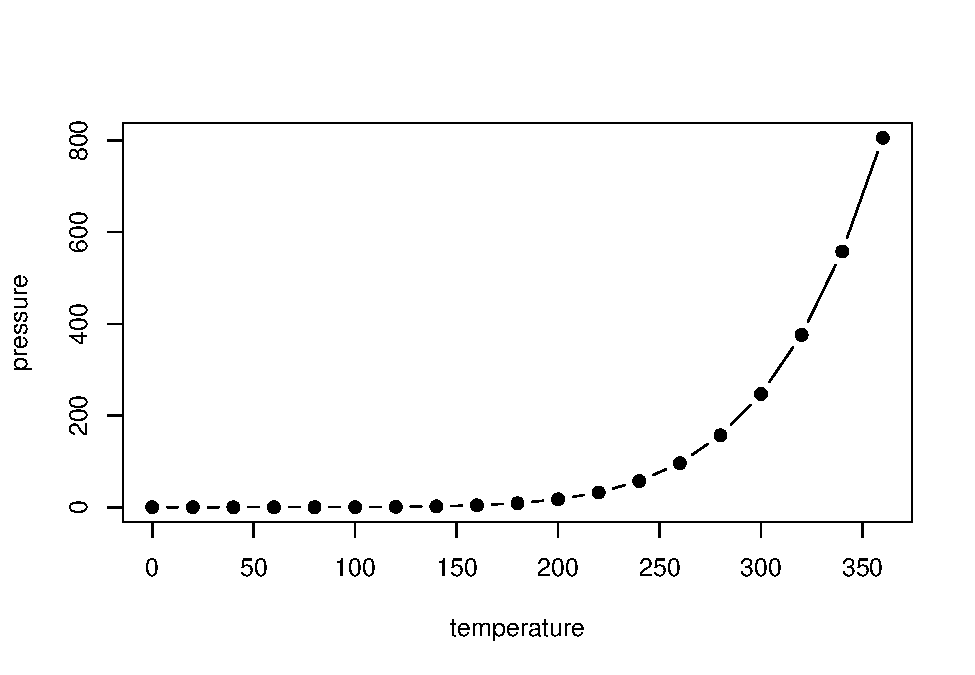
\includegraphics[width=0.75\linewidth]{03_results_files/figure-latex/pressure-1} 

}

\caption{An example figure.}\label{fig:pressure}
\end{figure}

And we can include image files directly, such as Figure \ref{fig:knitlogo}.

\begin{Shaded}
\begin{Highlighting}[]
\NormalTok{knitr}\SpecialCharTok{::}\FunctionTok{include\_graphics}\NormalTok{(}\StringTok{"img/mtcars{-}scatter.png"}\NormalTok{)}
\end{Highlighting}
\end{Shaded}

\begin{figure}

{\centering 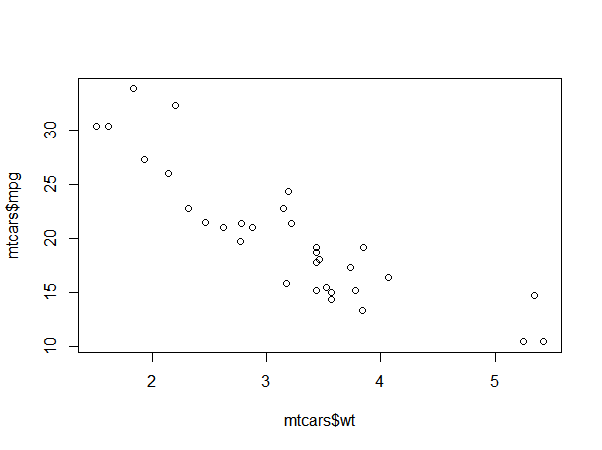
\includegraphics[width=0.75\linewidth]{img/mtcars-scatter} 

}

\caption{Another example figure.}\label{fig:knitlogo}
\end{figure}

To figure code chunks add the chunk option \texttt{fig.pos="H"} to use the LaTeX float package to try and position the figure where the code appears.

Also, this is how to reference a section, e.g.~the Introduction was chapter \ref{introduction} and the Literature Review was section \ref{literature-review}.

\hypertarget{discussion}{%
\chapter{Discussion}\label{discussion}}

\hypertarget{what-i-found}{%
\section{What I found}\label{what-i-found}}

\begin{itemize}
\tightlist
\item
  text 1
\item
  text 2
\item
  text 3
\item
  more text
\item
  more text
\end{itemize}

\hypertarget{what-it-means}{%
\section{What it means}\label{what-it-means}}

\begin{itemize}
\tightlist
\item
  text 6
\item
  text 7
\end{itemize}

\hypertarget{references}{%
\chapter{References}\label{references}}

\hypertarget{refs}{}
\begin{CSLReferences}{0}{0}
\leavevmode\hypertarget{ref-Abrams2005}{}%
\CSLLeftMargin{{[}1{]} }
\CSLRightInline{K. R. Abrams, C. L. Gillies, and P. C. Lambert. 2005. Meta-analysis of heterogeneously reported trials assessing change from baseline. \emph{Statistics in Medicine} 24, (2005), 3823--3844.}

\leavevmode\hypertarget{ref-hyndman2018forecasting}{}%
\CSLLeftMargin{{[}2{]} }
\CSLRightInline{Rob J Hyndman and George Athanasopoulos. 2018. \emph{Forecasting: Principles and practice}. OTexts.}

\end{CSLReferences}

\hypertarget{appendix-appendix}{%
\appendix}


\hypertarget{appendix-of-r-code}{%
\chapter*{Appendix of R code}\label{appendix-of-r-code}}
\addcontentsline{toc}{chapter}{Appendix of R code}

\begin{Shaded}
\begin{Highlighting}[]
\NormalTok{model }\OtherTok{\textless{}{-}} \FunctionTok{lm}\NormalTok{(y }\SpecialCharTok{\textasciitilde{}}\NormalTok{ x1 }\SpecialCharTok{+}\NormalTok{ x2, }\AttributeTok{data =}\NormalTok{ df)}
\FunctionTok{summary}\NormalTok{(model)}
\end{Highlighting}
\end{Shaded}


\backmatter

\end{document}
